\section{Co-occurence based multimodal recommender}
\label{sec:design}

The recommender we discuss will use past user behavior and metadata of items to compute the similarity between all items. Hence it is a hybrid recommender.
 
We use co-occurence to compute the similarity of two items. The recommenders looks up items that appear in the recent user history and presents the user a list with similar items.

All movies are stored as documents in a database (we use Apache Solr). The documents contain metainformation (e.g. title, tags, genre) about the items in fields. The fields are indexed by a search engine and made searchable.

In addidion the document has indicator fields. Indicator fields contain id's of that are found to be worth recommending in the co-occurence analysis.

The recommender discussed in this article has to parts.
\begin{description}
\item[Analysing User Input (offline)] In this part the user action are analised in order to compute the similarities of items. The similiarities are stored as indicators.
\item[Generate personalized recommendations (online)] A systems formats a list of recommended items.
\end{description}
We will first discuss the computation of similarities.


\subsection{Record user behavior}
\label{sec:inputdata}

\begin{figure}
  \centering
     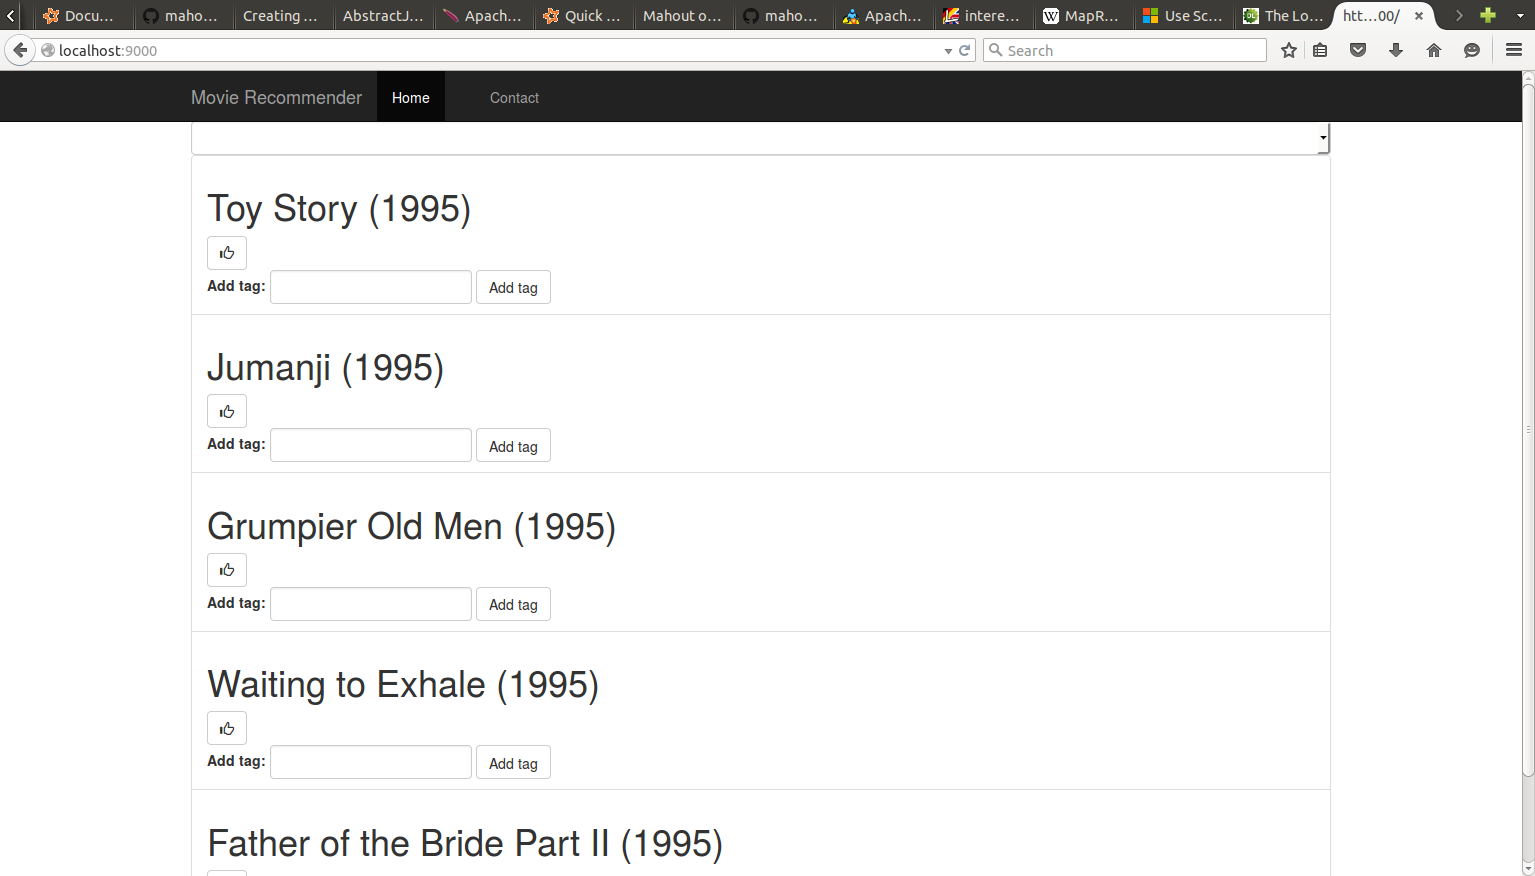
\includegraphics[width=0.9\textwidth]{collectinginput}
  \caption{The user can like and tag movies with the web front end. The user actions are recorded by the web server.}
  \label{fig:gui}
\end{figure}

The \gls{rec} suggests items that are similar to the ones the user already liked in the past. In order to build a model for similarity we need to train the recommender with some data about the items.
This section will descibe the type of input data we use  in our demo application. The report will refer to this type of input data. 

Many collaborative filtering recommender engines use excplicit user ratings to train their model. Explicit user ratings of a user for an item are expressed by numbers (e.g. a rating is a number between 1 and 5). The use of explicit feedback has some drawbacks.
\begin{itemize}
\item Only a small subset of users will rate items. This leads to a model that is skewed against user who like to rate.
\item The majority of ratings are associated with a small fraction of the most popular items \cite{Anderson}. As a result it is less likely that unknown items show up in the \gls{topn}. This behavior is undesirable because the goal of the recommender is to present items the a user would not find on his own.
\end{itemize}


Corresponding to \cite{Dunning14} the best choice of input data is the history of what a user actually does on a website. Hence the input data should consist of recorded \glspl{useraction} (e.g. purchase, view, like, tag).

In our demo web application we record two different user actions:
\begin{description}
\item[like]  Users can express their positive feedback for a movie by clicking on a ``like'' button (the \gls{like} action is an explicit rating. We use it instead of a purchase or view action in order to keep the GUI simple).
\item[tag] User can \gls{tag} items. Every item can be associated with a list of \glspl{tag}.
\end{description}
The recorded like and tag action are later used to compute similarity between items.
Figure \ref{fig:gui} shows the simplistic user interface of our demo web app.

The web browser sends every user action to the web server. The web server provides a REST Web API that receives the \glspl{useraction} as HTTP \verb|Post| request and saves them to a sqlite3 \footnote{https://www.sqlite.org/} database.

In order to analyse the data later we want to retrieve the action history $h_u$ for a particular user $u$ for a defined action and a list of tags for every item. Hence we have to structure the data accordingly. Figure \ref{fig:er} shows the entity relationship diagram for the user actions \gls{like} and \gls{tag}

\tikzset{multi  attribute/.style={attribute ,double  distance=1.5pt}}
\tikzset{derived  attribute/.style={attribute ,dashed}}
\tikzset{total/.style={double  distance=1.5pt}}
\tikzset{every  entity/.style={draw=blue , fill=blue!20}}
\tikzset{every  attribute/.style={draw=yellow, fill=yellow!20, node distance=1.0cm}}
\tikzset{every  relationship/.style={draw=red, fill=red!20}}

\begin{figure}
\centering
\begin{tikzpicture}[node distance=2.0cm]
  \node[entity](user){user};
  \node[relationship](like)[above right of=user]{ like } edge (user);
  \node[attribute](date2)[above of=like]{ date } edge (like);
  \node[entity](item)[below right of=like]{item} edge (like);
  \node[relationship](tag)[below right of=user]{ tag } edge (user) edge (item);
  \node[attribute](text)[below right of=tag]{ text } edge (tag);
  \node[attribute](date1)[below left of=tag]{ date } edge (tag);
  \end{tikzpicture}
\caption{The data model allows us to retrieve the action history for every user. Like and tag form associations of user with item.}
\label{fig:er}
\end{figure}

It makes sense to start recording behavioral data month's before depoying the recommender engine because the recommender engine has to analyze the data and build a model of similarty among items in order to create personalized recommendations.

\subsection{How to compute the top-N recommendations list?}
\label{sec:problem}
This section gives a mathematical description of the top-N recommendation task and hence it describes the computations required to produce recommendations. The description refers to the \gls{rec}.

Suppose we have a metric to express similarity between two items as a numerical value and the magnitude of the value determines the strength of similarity. If we compute the similarity for every item pair in a set of $n$ items, we can represent the result in a matrix $M$. $M$ is a $n \times n$ matrix. Each row and each column contains the similarities between one particular item and all other items. $M$ is symetric across the diagonal because the similarity between $a$ and $b$ must be the same as between $b$ and $a$ (commutativity). The diagonal of $M$ contains the value for maximum similarity because this value represents the comparison of an item to itself. $M$ is called the \gls{indicatorm}. Equation \ref{eq:similaritymatrix} shows an example of an \gls{indicatorm} with 4 items.

\begin{equation}
  \label{eq:similaritymatrix}
M =\bordermatrix{~ & 1 & 2 & 3 & 4 \cr
 1 & 1  & 0.40 & 0.9 & 0.1 \cr
2 & 0.40 &1  & 0.9 & 0.1 \cr
 3& 0.9 & 0.9 &1  & 0.63 \cr
 4 & 0.1 & 0.1 & 0.63 &1  \cr}
\end{equation}
Further we represent a user action history for each user as vector $h_l$ of length $n$. $h_l$ contains an element for every item. The user's interactions with an item are represented as binary values in $h_l$. If the there is an interaction with an item in the history the value or the corresponding element is 1. Otherwise the value is 0. For example equation \ref{eq:history} shows a user's action history for the action ``like''. He has liked item 1 and 2.

\begin{equation}
\label{eq:history}
h_l =
\begin{pmatrix}
 1 \\
 1 \\
 0 \\
 0 \\
\end{pmatrix}
\end{equation}

To create a \gls{topn} for user $u$ we compute the matrix vector product of $M$ and $h_l$. The result $r$ is a vector of length $n$, that contains a value for every item. $r$ maps every item to a value that indicates how likely an item is of interest to user $u$. According to equation \ref{eq:recommendation} item 3 correspond to the best recommendation.

\begin{align}
  \label{eq:recommendation}
r_u &= M h_u 
&=
\begin{pmatrix}
  1  & 0.40 & 0.9 & 0.1 \\
 0.40 &1  & 0.9 & 0.1 \\
  0.9 & 0.9 &1  & 0.63 \\
  0.1 & 0.1 & 0.63 &1 \\  
\end{pmatrix} 
\begin{pmatrix}
 1 \\
 1 \\
 0 \\
 0 \\
\end{pmatrix}
&= 
\begin{pmatrix}
 1.4 \\
 1.4 \\
 1.8 \\
 0.2 \\
\end{pmatrix}
\end{align}

In order to create the complete \gls{topn} based on the vector $r$ we create a list of all item the user hasn't seen (the ones with zeros in $h_u$) and sort the list according the values in $r$. Items with a high value appear first in the list. In other words we return a ranked list of items. This list forms the \gls{topn}. In the example of equation \ref{eq:recommendation} the recommender would return item 3 followed by item 4. Item 1 and to are removed because the apear in the user's history.

\subsection{How to measure similarity among items?}
\label{sec:llr}

In section \ref{sec:problem} we use a matrix $M$ that contains similarity strength among items. This section describes how $M$ is computed.

In order to compute the similarity between two items \cite{Dunning14} proposes to count the \gls{coocc} among two items with respect to a particular user action and then compute the the \gls{llr} ratio of that \gls{coocc}.

\gls{coocc} is the number of times a pair of items appear together in some user's action history. For instance, if there are 5 users who purchased both items $A$ and $B$ then $A$ and $B$ co-occur 5 times. \gls{coocc} is indicates similarity. The more two items turn up togheter, the more related they probably are.

The \gls{llr} ratio is a probabilistic measure of the importance of a \gls{coocc}. 

Co-occurence in the context of the recommender engine could be user-item interaction (like, purchase, etc) and tag-item associations is the number of same users that interact with them.

According to \cite{Dunning93} the log-likelihood similiarity is suitable for data that only captures the interaction and no preference values between users and items. 
Compared to the Jaccard coefficient \cite{Hartung} the log-likelihood-based similarity computes higher similarites for anomalous co-occurences than for items that occur in every user history. The log-likelihood similarity  is the probability that two users share the same items because the items are similar and not due to chance. It finds important cooccurence and filters out the coinidental. For a detailed explanation of the math involved see appendix and \cite{Dunning93}. 

We describe the log-likelihood-based similarity with a small example dataset. Suppose we analyse the following web log of user purchases represented as a table (see appendix of raw web log).

\begin{table}
\begin{center}
\begin{tabular}{rllll}
 & 101 & 102 & 103 & 104\\
1 & x & x & x &  \\
2 & x &   & x & x\\
3 & x & x & x &  \\
4 &   & x & x & x\\
5 & x & x & x & x\\
\end{tabular}
\end{center}
\caption{Example dataset. The columns represent the user interaction with an item. Items are named 1 - 4 and users 101 - 104}
\label{tbl:llr}
\end{table}

Table \ref{tbl:llr} shows the purchases of four users for five items. The items are represented with ids 1-4 and the users with ids 101 - 104.
In the example dataset of table \ref{tbl:llr} the items 1 and 2 are similar because they were purchased by the same users. 

In order to get the similarities between all items we count the \gls{coocc} of purchases for all item pairs. This leads to the \gls{indicatorm} shown in table \ref{tab:cooccurencematrix}.

\begin{table}
  \centering
\begin{center}
\begin{tabular}{rrrrrr}
  & 1 & 2 & 3 & 4 & 5\\
1 & 4 & 2 & 3 & 2 & 3\\
2 & 2 & 3 & 2 & 1 & 3\\
3 & 3 & 2 & 3 & 2 & 3\\
4 & 2 & 1 & 2 & 3 & 3\\
5 & 3 & 3 & 3 & 3 & 4\\
 &  &  &  &  & \\
\end{tabular}
\end{center}
  \caption{Co-occurence matrix for item purchases}
  \label{tab:cooccurencematrix}
\end{table}

In the next step we compute the log-likelihood ratio strength of the \glspl{coocc} for every item pair. This will produce a $5 \times 5$ \gls{indicatorm}. Table \ref{tab:indicatormatrix} shows the \gls{indicatorm} for the sample dataset from table \ref{tbl:llr}

\begin{table}
  \centering
\begin{center}
\begin{tabular}{rrrrrr}
  & 1 & 2 & 3 & 4 & 5\\
1 &   & 0.40 & 0.81 & 0.63 & 0\\
2 & 0.40 &  & 0.40 & 0.63 & 0\\
3 & 0.81 & 0.40 &  & 0.63 & 0\\
4 & 0.63 & 0.63 & 0.63 &  & 0\\
5 & 0 & 0 & 0 & 0 & \\
 &  &  &  &  & \\
\end{tabular}
\end{center}
  \caption{Indicator matrix for item purchases}
  \label{tab:indicatormatrix}
\end{table}

Allthoug item 5 share all users with item 1 and 3, the log-likelihood ratio is 0. Every user purchased item 5. It would not be interesting to recommend item 5 to a user because it is to obious.

\begin{figure}
\centering
\begin{tikzpicture}[node distance=40mm,
data/.style={
rectangle,
draw,
thin,
minimum height=3.5em
},
to/.style={->,>=stealth',shorten >=1pt,semithick,font=\footnotesize},
]
\node (hist) [data, align=left] {User actions\\history};
\node (co) [data,right of=hist,align=left] {Co-occurence};
\node (in) [data,right of=co,align=left] {LLR\\indicator\\matrix};
\draw[to] (hist) -- (co);
\draw[to] (co) -- (in);
\end{tikzpicture}
\caption{To compute the indicator matrix {\ttfamily spark-itemsimilarity} computes the co-occurence  of user actions and then compute the indicator matrix with the log-likelihood strengths.}
\end{figure}


\subsubsection{Log-likelihood similarity implementation}
\label{sec:llrimpl}

Apache Mahout provides an implemenation of log-likelihood similarity with the class \verb|LogLikelihoodSimilarity|. Unfortunatly the \verb|LogLikelihoodSimilarity| is a non-distributed implementation. It would take too long to calculate the indicator matrix for a dataset with over 10 million items and we would have difficulties to load all data into the memory. 

The computation of the \gls{coocc} of every item pair can be distributed by applying the MapReduce programming model as follows:
\begin{description}
\item[Map] Determine all \glspl{coocc} for one user's history and yield a pair of items for each \gls{coocc}
\item[Reduce] Count for each item all \glspl{coocc} and yield a vector with all items and the corresponding \gls{coocc}.
\end{description}
\todo{bild map reduce einfuegen}

This task can run in parallel on different nodes on a cluster computer framework, such as Apache Spark. Hence the computation of the \gls{indicatorm} is \gls{scalable}.
In order to compute the \gls{llr} similarity distributed, Apache Mahout provides the \verb|spark-itemsimilarity| job. \verb|spark-itemsimilarity| connects to a Spark cluster and computes the \gls{indicatorm} in parallel.  With the \verb|spark-itemsimilarity| job the indicator matrix can be computed in $O(n)$ \cite{Schelter}. 

Apache Spark is a cluster computer framework. It allows user programs to load data into a cluster's memory. It is well suited to machine learning algorithms \cite{Karau}.

To run \verb|spark-itemsimilarity| we have to deploy Apache Spark and and start it in standalone mode with the script \verb|start-master.sh|. Once startet the script will print a URL which we can pass the \verb|spark-itemsimilarity| job as ``master'' argument and the job can connect to the cluster. \verb|spark-itemsimilarity| is a command line job and we can start it from the mahout shell.

\begin{verbatim}
./mahout spark-itemsimilarity --input $infile --output $outfile
\end{verbatim}

The input text file has to be in the following format:
\begin{verbatim}
userID, action, itemID
\end{verbatim}
\verb|spark-itemsimilarity| will output an indicator matrix created by collecting and counting all \glspl{coocc} and calculating the \gls{llr} ratio strenght. The output will be a text file that represents the indicator matrix as sparse vectors for every item. For every item we get the similarities to all other items.
\begin{verbatim}
itemID1<tab>itemID2:similarityvalue<space>itemID3:similarityvalue
\end{verbatim}

In our demo application we have written a python script to fetch the data from the sqlite3 database and transform to the Spark input format.
The co-occurence based recommender uses the user behavior log in order to compute a similarity model. 

\begin{figure}
\centering
\begin{tikzpicture}[node distance=40mm,
data/.style={
rectangle,
draw,
thin,
minimum height=3.5em
},
to/.style={->,>=stealth',shorten >=1pt,semithick,font=\footnotesize},
]
\node (log) [data, align=left] {User actions\\log file};
\node (spark) [data,right of=log,align=left] {Apache Spark\\LLR job};
\node (model) [data,right of=spark,align=left] {Similarity\\model};
\draw[to] (log) -- (spark);
\draw[to] (spark) -- (model);
\end{tikzpicture}
\caption{The {\ttfamily spark-itemsimilarity} job of Apache Spark computes the LLR similarity based on the user behavior log file.}
\end{figure}

\subsection{Using more than one type of behavior}
\label{sec:multimodal}

Most collaborative filtering algorithm use only explicit or implicit ratings to compute similarity.
But we can improve the performance of the recommender engine by using multiple types of user actions. In addition to likes we could use tag-associations to compute the similariy. In table \ref{tab:llr} we count co-occurence of items in a user' purchase action history. Instead of the action history we could use tags that are associated items. We count the co-occurence of items associated with a tag. This. 

Suppose we compute a \gls{indicatorm} based on likes $M_l$ and one based on tag associations $M_t$. An $h_l$ is a user's history of ``likes'' and $h_t$ is the user's tag history. Then we can compute the recommendations $r$ with

\begin{equation}
  \label{eq:multi}
  r = h_l M_l + h_t M_t
\end{equation}

In our demo web application we use ``likes'' and tags but virtually all user actions can be used to improve the recommendation

\subsection{Apache Solr}
\label{sec:solr}

Before we describe why we use a the search engine Apache Solr to deploy a recommendation engine, we give a short introduction to Apache Solr.

Apache Solr is a search engine that is optimized to search large volumes of text-centric data and return results sorted by relevance. It is built on Apache Lucene, an information retrieval library \cite{grainger}. Solr stores the documents in a flat structure and we can search for terms in the documents.
Solr returns documents sorted in descending order by a score that indicates the strength of the match of the document to the query. In a relational database a row either matches a query or it does not. That is the reason why a search engine is more suitable for our use case.

The reason why we deploy a search engine in order to make recommendations is that Solr scores documents based on the presence of query terms in the document similar to a recommendations engine based on the presence of indicator.

\subsection{Connection of a recommender and a search engine}
\label{sec:relation}

A common approach to users for coming up with good queries is to think of words that would likely appear in a relevant document, and to use those words as query.

There are similarities between weighting of indicator scores and the mathematics that underlie text retrival engines

Let's say we represent the recommendations for a user as a vector $r$. The elements of $r$ are floating point number which represent preferences for all items for a user. Most collaborative filtering type recommenders compute $r$ by multiplying the given preferences of a user $h_u$ with the indicator matrix $M$ for all items. In our example $M$ contains the similarity values of the log-likelihood cooccurence.

\begin{equation}
  \label{eq:cf}
  r = h_u M
\end{equation}

Equations \ref{eq:cf} actually means to compare the user history $h_u$ to the rows of the indicator matrix $M$. This result in a vector $r$ containing a score that indicates the strength of the match of the item to the history $h_p$. The recommender ranks the items by the score and presents them to the user. These items form the recommendations.

This is exactly what the ranked retrieval feature of a search eninge does.
The user history $h_U$ is the query. The items are the documents. And the text of the fields contain similar items.

In addition we can use TF-IDF \cite{Manning} weighting to mitigate popular items.

This is why we deploy Solr to build a recommender.

We store all items as documents in Solr. The documents contain the metadata like (title, genre, tags, etc). In addidtion we populate a filed for every indicator with the similar item ID's discovered with the coocuccence similartiy from section \ref{sec:llr}.

\begin{lstlisting}[caption={Item metadata and similar items are stored in Solr.},label={lst:solrdoc}]
{
    "id": "1",
    "title": ["Toy Story (1995)"],
    "tags":"Pixar animation fantasy",
    "likeindicator": "1688 1834 3893 4366 6281 33162 50872 53000 ",
    "_version_": 1505056335358591000
}
\end{lstlisting}

In order to build a recommender using a search engine we store the output of the co-occurence analysis in Solr. The search engine actually delivers the recommendations to our users.

\subsection{Retrieve recommendation}

In order to produce recommendations we compose a Solr query from the user history. The user history is stored in the web log. The web server sends this query to Solr. Solr responds with a ranked result set. The web server then formats the response from Solr and sends a list of recommended items to the user.

\begin{figure}
\centering
\begin{tikzpicture}[node distance=20mm,
data/.style={
rectangle,
draw,
thin,
minimum height=3.5em
},
to/.style={->,>=stealth',shorten >=1pt,semithick,font=\footnotesize},
]
\node (web) [data] {Web server};
\node (log) [data,below of = web, align=left] {User actions\\log file};
\node (browser) [data,left of=web,node distance=50mm] {Webbrowser};
\node (solr) [data,right of=web,node distance=50mm] {Search engine};
\draw[to] (web) -- (log);
\draw[to] (browser) -- node[midway,above] {user actions} (web);
\end{tikzpicture}
\caption{The web server sends this query to Solr. Solr responds with a ranked result set.}
\end{figure}


Another reason why we deploy a search engine is that the application is read-dominant. The recommender will query the data far more often than it will create new documents or update the indicators. Solr is optimized to for executing queries as opposed to storing data.

Solr is used in the offline and the online part of the recommendation engine.
The items and their corresponding similarity indicators from the Apache Spark job are stored with Apache Solr. 

\subsection{Parameters}
\label{sec:parameters}

This section descripes the paratemter of the recommender discussed in this report.
\begin{description}
\item[similarity threshold] We have to define a threshold to separate similar items occording to the LLR similarity from the rest (e.g. 0.5).
\item[user history to consider] We retrieve recommendations with a part of the user history. We have to define the number of log entries to consider.
\end{description}

\subsection{Two-parts design}

The recommender described in this article is divided in two parts.
\begin{itemize}
\item Computation of simililarity and the update of the text search engine is done offline, ahead of time.
\item Recommendations are generated instantly by quering the text search engine using rescents actions of the user.
\end{itemize}
